\documentclass[10pt,twocolumn,letterpaper]{article}

\usepackage{iccv}
\usepackage{times}
\usepackage{epsfig}
\usepackage{graphicx}
\usepackage{amsmath}
\usepackage{amssymb}
\usepackage{float}
\usepackage{subfigure}
\usepackage{multirow}
\usepackage{array}

% Include other packages here, before hyperref.
\newcommand{\PreserveBackslash}[1]{\let\temp=\\#1\let\\=\temp}
\newcolumntype{C}[1]{>{\PreserveBackslash\centering}p{#1}}
% If you comment hyperref and then uncomment it, you should delete
% egpaper.aux before re-running latex.  (Or just hit 'q' on the first latex
% run, let it finish, and you should be clear).
\usepackage[pagebackref=true,breaklinks=true,letterpaper=true,colorlinks,bookmarks=false]{hyperref}

\def\comm[#1]{{\small \textcolor{red}{\emph{#1}}}}
\def\red[#1]{\textcolor{red}{\textbf{#1}}}
\def\redn[#1]{\textcolor{red}{#1}}
\def\blue[#1]{\textcolor{blue}{#1}}
\def\green[#1]{\textcolor{green}{#1}}
\def\revise[#1]{{\small \textcolor{blue}{\emph{}}}}

% \iccvfinalcopy % *** Uncomment this line for the final submission

\def\iccvPaperID{621} % *** Enter the ICCV Paper ID here
\def\httilde{\mbox{\tt\raisebox{-.5ex}{\symbol{126}}}}

% Pages are numbered in submission mode, and unnumbered in camera-ready
\ificcvfinal\pagestyle{empty}\fi
\begin{document}

%%%%%%%%% TITLE
\title{Face Sketching with Deep Neural Networks}

\author{First Author\\
Institution1\\
Institution1 address\\
{\tt\small firstauthor@i1.org}
% For a paper whose authors are all at the same institution,
% omit the following lines up until the closing ``}''.
% Additional authors and addresses can be added with ``\and'',
% just like the second author.
% To save space, use either the email address or home page, not both
\and
Second Author\\
Institution2\\
First line of institution2 address\\
{\tt\small secondauthor@i2.org}
}

\maketitle
%\thispagestyle{empty}

%%%%%%%%% ABSTRACT
\begin{abstract}

In this paper, we propose a new face sketch synthesis framework based on deep neural networks. Imitating the process of how artists draw sketches, our framework synthesizes face sketches in a cascaded manner in which a content image is first generated that outlines the shape of the face and key facial features, and textures and shadings are then added. By exploiting the capability of deep networks for generating beautiful textures and stylized images, our framework can produce sketches that look like sketches drawn by real artists in strokes. Experiments are carried out on both the CUHK and AR datasets. Quantitative and qualitative evaluations suggest that our framework outperforms other state-of-the-arts methods.
\end{abstract}

%%%%%%%%% BODY TEXT
{
\section{Introduction}
}
Face sketch synthesis has drawn a great attention from the community in recent years because of its wide range of applications. For instance, it can be exploited in law enforcement for identifying suspects from a mug shot database consisting of both photos and sketches. Besides, face sketch has also been widely used for entertainment purpose. For example, filmmakers could employ face sketch synthesis technique to ease the cartoon production process. \par
Unfortunately, there exists no easy solution to face sketch synthesis due to the big stylistic gap between photos and sketches. In the past two decades, a number of exemplar based methods~\cite{wang2009face,zhang2010lighting,zhou2012markov} were proposed. In these methods, an input photo is divided into patches and candidate sketches for each photo patch are selected from a training set. The sketch output of a photo patch can be represented by either the best candidate or a linear combination of the best $K$ candidate sketch patches. However, processing each photo patch individually often introduces inconsistency between neighboring patches. To tackle this problem, methods in~\cite{wang2009face,zhang2010lighting,zhou2012markov} adopted Markov Random Fields (MRF) to regularize the synthesis process. Recently, an image based approach~\cite{song2014real} based on the idea of joint image filtering was proposed. It was found superior in suppressing noises in the sketch. Another recent approach based on a feed-forward convolutional neural network (FCNN) was found to be more effective in generating discriminative facial details~\cite{zhang2015end}. Although sketches produced by these methods do look like the faces in the photos, they look quit different from sketches drawn by real artists. One major reason is that these methods do not consider the style of the synthesized sketches. For example, the hair in their synthesized sketches is often lack of texture, and the region around the face boarders often suffers from blurring artifacts (see Fig.~\ref{fig:example_comp}). Besides, both the exemplar based and image based approaches cannot handle structures that do not exist in the training set (e.g., clothes in Fig.~\ref{fig:example_comp}).\par
% \begin{figure}[t]
% \centering
% \begin{minipage}[t]{0.24\linewidth}
% \centering
% 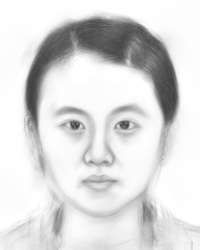
\includegraphics[width=1\linewidth]{example_ssd.pdf}
% \cite{song2014real}
% \end{minipage}
% \begin{minipage}[t]{0.24\linewidth}
% \centering
% 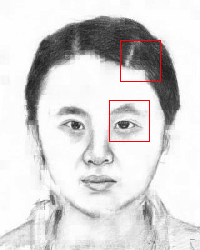
\includegraphics[width=1\linewidth]{example_mrf.pdf}
% \cite{wang2009face}
% \end{minipage}
% \begin{minipage}[t]{0.24\linewidth}
% \centering
% 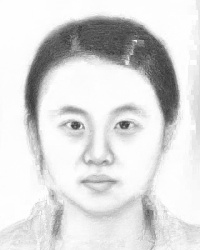
\includegraphics[width=1\linewidth]{example_wmrf.pdf}
% \cite{zhou2012markov}
% \end{minipage}
% \begin{minipage}[t]{0.24\linewidth}
% \centering
% 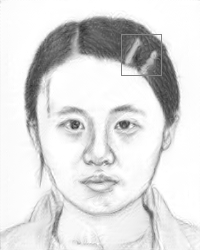
\includegraphics[width=1\linewidth]{example_ours.pdf}
% Proposed
% \end{minipage}
% \caption{Face sketches generated by existing methods and the proposed method. The proposed method can achieve a better performance than the exemplar based methods~\cite{wang2009face,zhou2012markov} and the image based method~\cite{song2014real} in appearance.}
% \label{fig:example_comp}
% \end{figure}
Inspired by the way how artists draw sketches, we propose a new framework for face sketch synthesis that can overcome the aforementioned limitations. For an artist, instead of drawing sketches region by region, the procedure of sketching a face usually starts with outlining the shape of the key facial features like the nose, eyes and mouth. Textures and shadings are then added to regions such as hair lips, and bridge of the nose to give sketches a specific style. In our method, the outline of a face is delineated by a feed-forward neural network, and textures and shadings are then added by a style transfer approach.  We formulate the style as a statistical measure of the features extracted from multiple resolutions of the sketches using the VGG-Network~\cite{simonyan2014very}. Due to the non-linearity of these features and the fact that there usually does not exist a training photo that is very similar to the test photo, estimating the style for a target sketch is not easy. In spired by the work of Wang and Tang~\cite{wang2009face}, we divide the feature maps of the target sketch into a grid and use the features of a candidate sketch patch as a surrogate for the feature map patch of a grid cell. A target style is then computed from the resulting feature maps. Our approach is superior to the current state-of-the-art methods in that (1) it is capable of generating more stylistic sketches without introducing over smoothing artifacts and (2) it can draw structures which do not exist in the training set.\par
{
\section{Related Work}
}
{
\subsection{Face Sketch Synthesis}
}
Based on the taxonomy of previous studies~\cite{song2014real,zhou2012markov}, face sketch synthesis methods can be roughly categorized into profile sketch synthesis methods~\cite{berger2013style,chen2001example,xu2008hierarchical} and shading sketch synthesis methods~\cite{liu2005nonlinear,song2014real,tang2003face,wang2009face,zhang2015end,zhang2010lighting,zhou2012markov}. Compared with profile sketches, shading sketches are more expressive and thus more preferable in practice. Based on the assumption that there exists a linear transformation between a face photo and a face sketch, the method in~\cite{tang2003face} computes a global eigen-transformation for synthesizing face sketches from face photos. This assumption, however, does not always hold since the modality of face photos and that of face sketches are quite different. Fortunately, Liu et al.~\cite{liu2005nonlinear} found that the linear transformation holds better locally and therefore they proposed a patch based method to perform sketch synthesis. A MRF based method~\cite{wang2009face} was proposed to preserve large scale structures across sketch patches. Variants of the MRF based methods were introduced in~\cite{zhang2010lighting,zhou2012markov} to improve the robustness to lighting and pose, and to render the ability of generating new sketch patches. In addition to these MRF based methods, approaches based on guided image filtering~\cite{song2014real} and feed-forward convolutional neural network~\cite{zhang2015end} are also found to be effective in transferring photos into sketches.
{
\subsection{Style Transfer with Convolution Neural Network}
}
The class of Convolutional Neural Networks (CNN) is perhaps the most powerful tool in image processing. It usually contains layers of filters each of which extracts a certain feature from the input or from the output of the previous layer. The VGG-Network~\cite{simonyan2014very}, one popular instance of such networks, rivals human performance in image classification tasks. This demonstrates the ability of CNN in feature extraction. In~\cite{gatys2015texture,gatys2015neural}, Gatys et al. studied the use of CNN in style representation where a target style is computed based on features extracted from an image using the VGG-Network and an output image is generated by minimizing the difference between its style and the target style. Likewise, a perceptual loss function measuring the difference in style between a targeting image and images generated from a CNN was proposed in~\cite{feifei2016} and it was then exploited in the CNN training stage. Our style transfer mechanism is inspired by but different from these works~\cite{gatys2015texture,gatys2015neural,feifei2016} in that our target style is extracted from many images rather than from a single style image. Note that there usually does not exist a single style image in the training set that matches all properties of the test image. Hence, we propose computing the target style based on multiple images. The difficulty of generating a target style from multiple images lies in the non-linearity of the neural network.
%-------------------------------------------------------------------------

{
\section{Overview of Our Method}
}
% \begin{figure*}[t]
% \centering
% \subfigure[]{
% 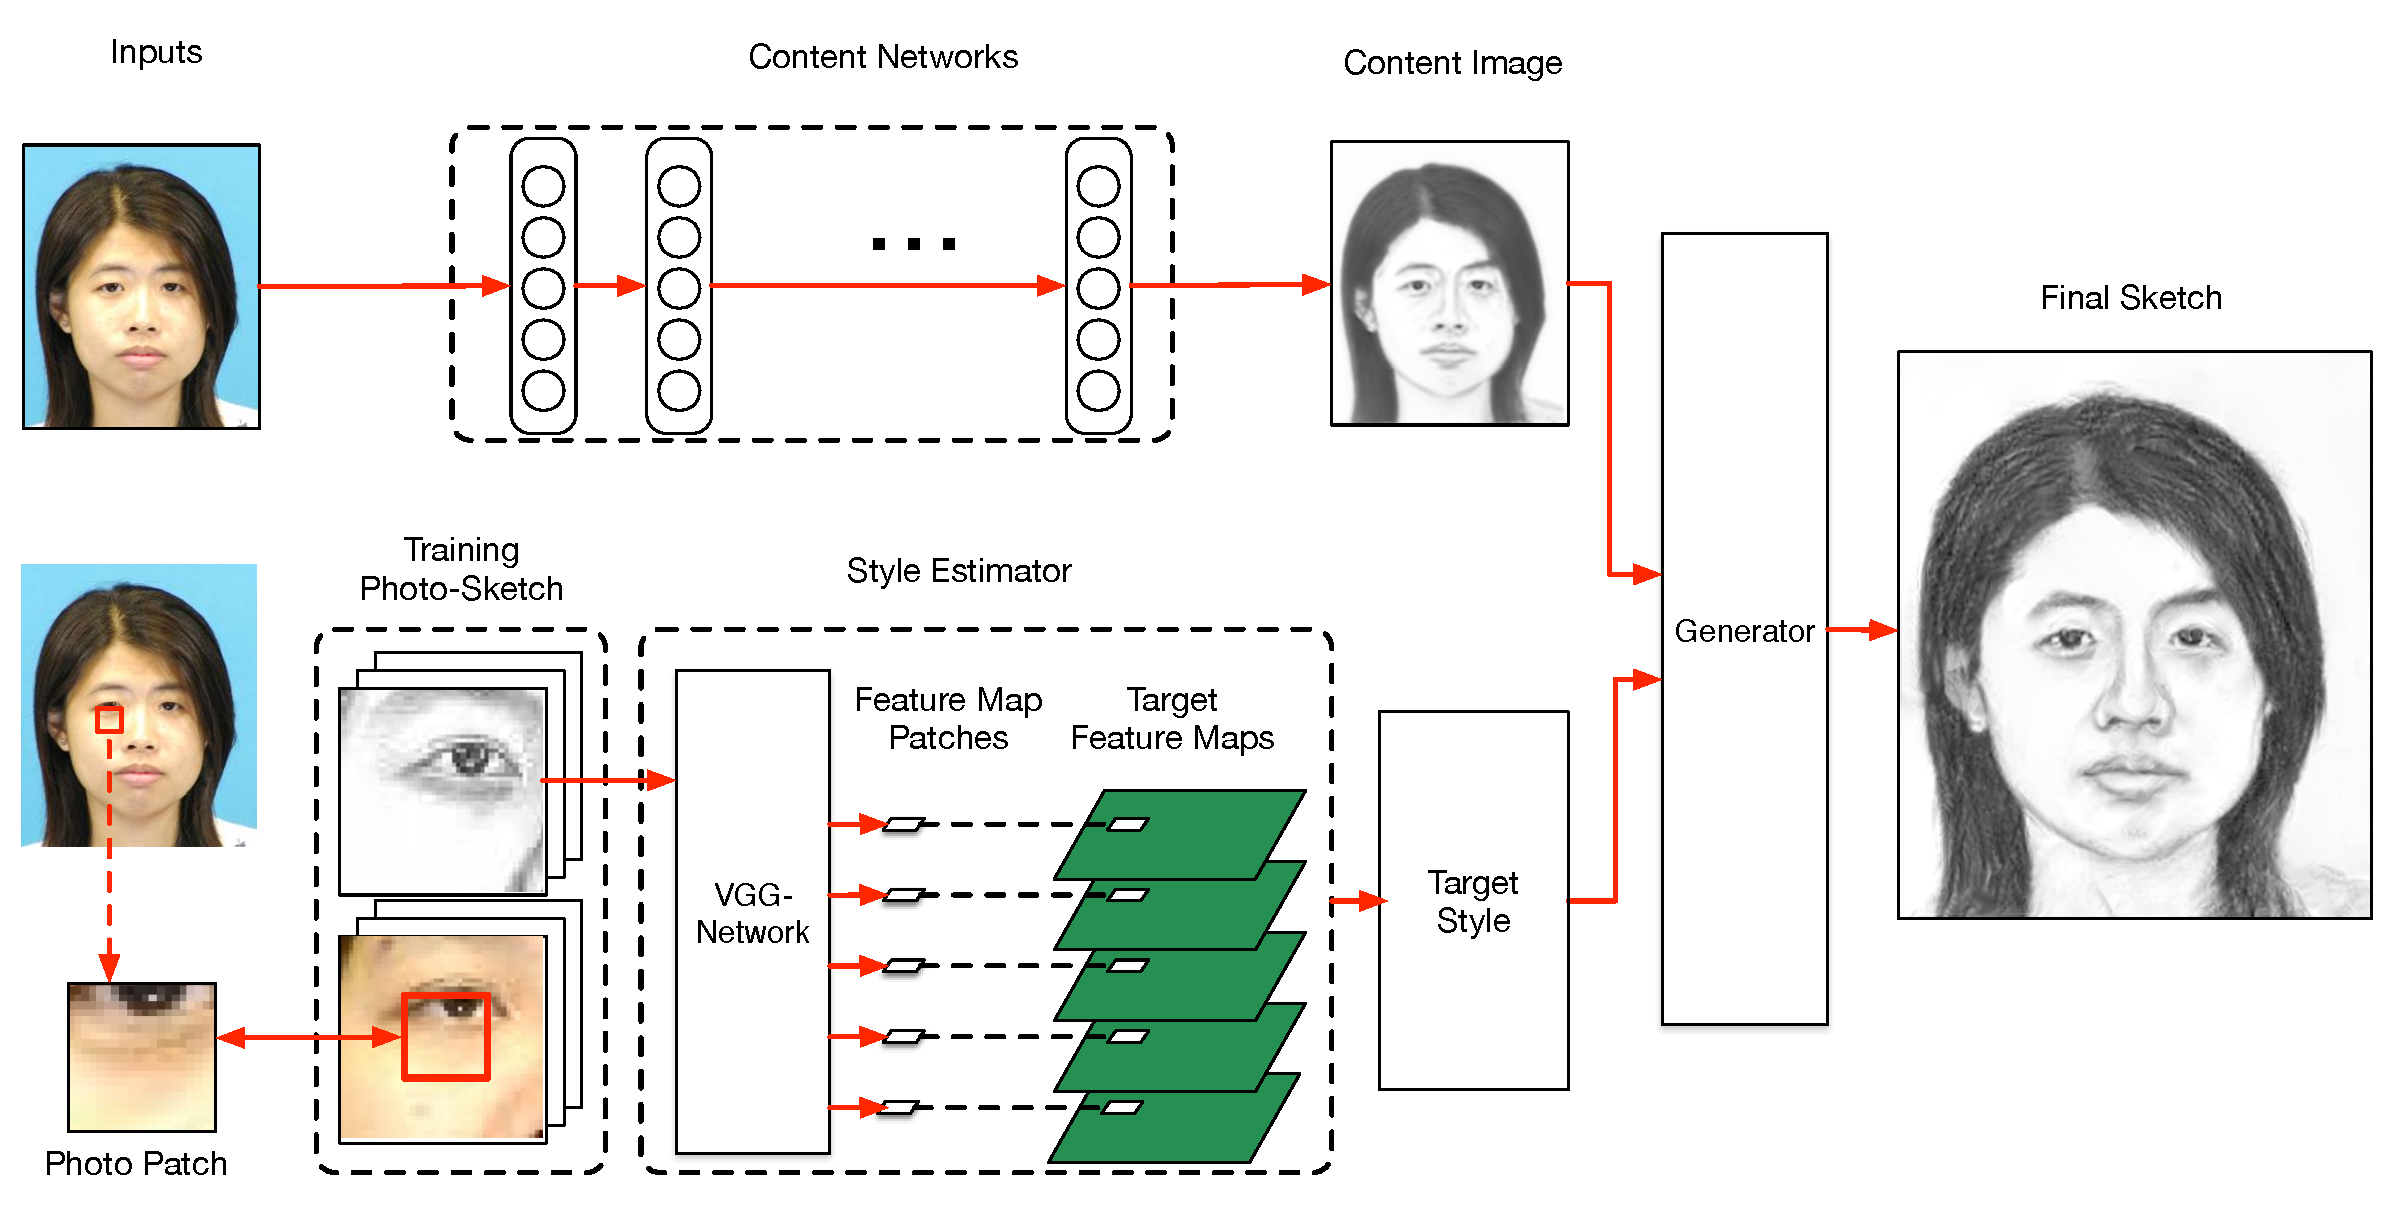
\includegraphics[width=0.85\linewidth]{overview.pdf}
% }
% \caption{The proposed method contains two branches which take an photo aligned by the eyes as inputs. The content network outputs a content image and the style estimator generates a target style. The final sketch is generated by combing the target style with the content image.}
% \label{fig:overview}
% \end{figure*}
Our method can be classified as a shading synthesis method. The steps of our method are summarized in Fig.~\ref{fig:overview}. First, a preprocessing step as described in~\cite{wang2009face} is carried out for all photos and sketches in a training set to align the centers of two eyes. A test photo $\mathcal{I}$ is then fed into two branches, namely the content network and the style generator, respectively. The content network converts the test photo into a content image $\mathcal{C}$, where facial features and the shape of the face are outlined with the global arrangement of the facial features preserved. It is not necessary that the style of the content image resembles a real sketch, but the shapes of different features such as noses, eyes, mouthes and hair, should be delineated. The style estimator takes the test photo as input and utilizes photo-sketch pairs in the training set to generate a target style $\mathcal{S}$ which we want to transfer to the final sketch. Given $\mathcal{C}$ and $\mathcal{S}$, we generate a sketch $\mathcal{X}$ that combines the content information in $\mathcal{C}$ with the style representation $\mathcal{S}$. This is formulated as an optimization problem over an energy function taking both $\mathcal{C}$ and $\mathcal{S}$ into considerations. Details will be explained in the following subsections.
{
\section{Content Image Generation}
}
We use CNN to build our content network (see Fig~\ref{fig:content_NN}). In addition to the test photo, two location channels containing spatial information (i.e., x and y coordinates) and a difference of Gaussian (DoG) channel containing edge information are fed into the content network. As pointed out in~\cite{wang2009face}, face sketch synthesis algorithms benefit from integrating features from multiple resolutions. We employ an inception module inspired by the GoogLeNet~\cite{szegedy2015going} to extract features. It concatenates feature maps generated from filters with different spatial resolutions. Our inception unit contains $3$ CNN filter groups, with each group having $32$ filters. The filters in these 3 groups have a size of $autoref(1\times1)$, $autoref(3\times3)$ and $autoref(5\times5)$ respectively (see Fig. 3(b)). The output features are then fed to a three-layer-CNN for feature integration, where the size of all filters are fixed at $autoref(1\times1)$. Finally, the integrated features are used to reconstruct the content map by a two-layer-CNN with the filter size being $3\times3$. A mirror padding is carried out before the convolution operation when necessary to ensure the output feature map is the same size as the input. It is observed that the output of the content net outlines the shapes of the facial features, but its style does not look like sketches. For example, there exists no texture in the hair region and there is a lack of shadings to convey 3D information.
% \begin{figure*}[htbp]
% \centering
% \subfigure[]{
% 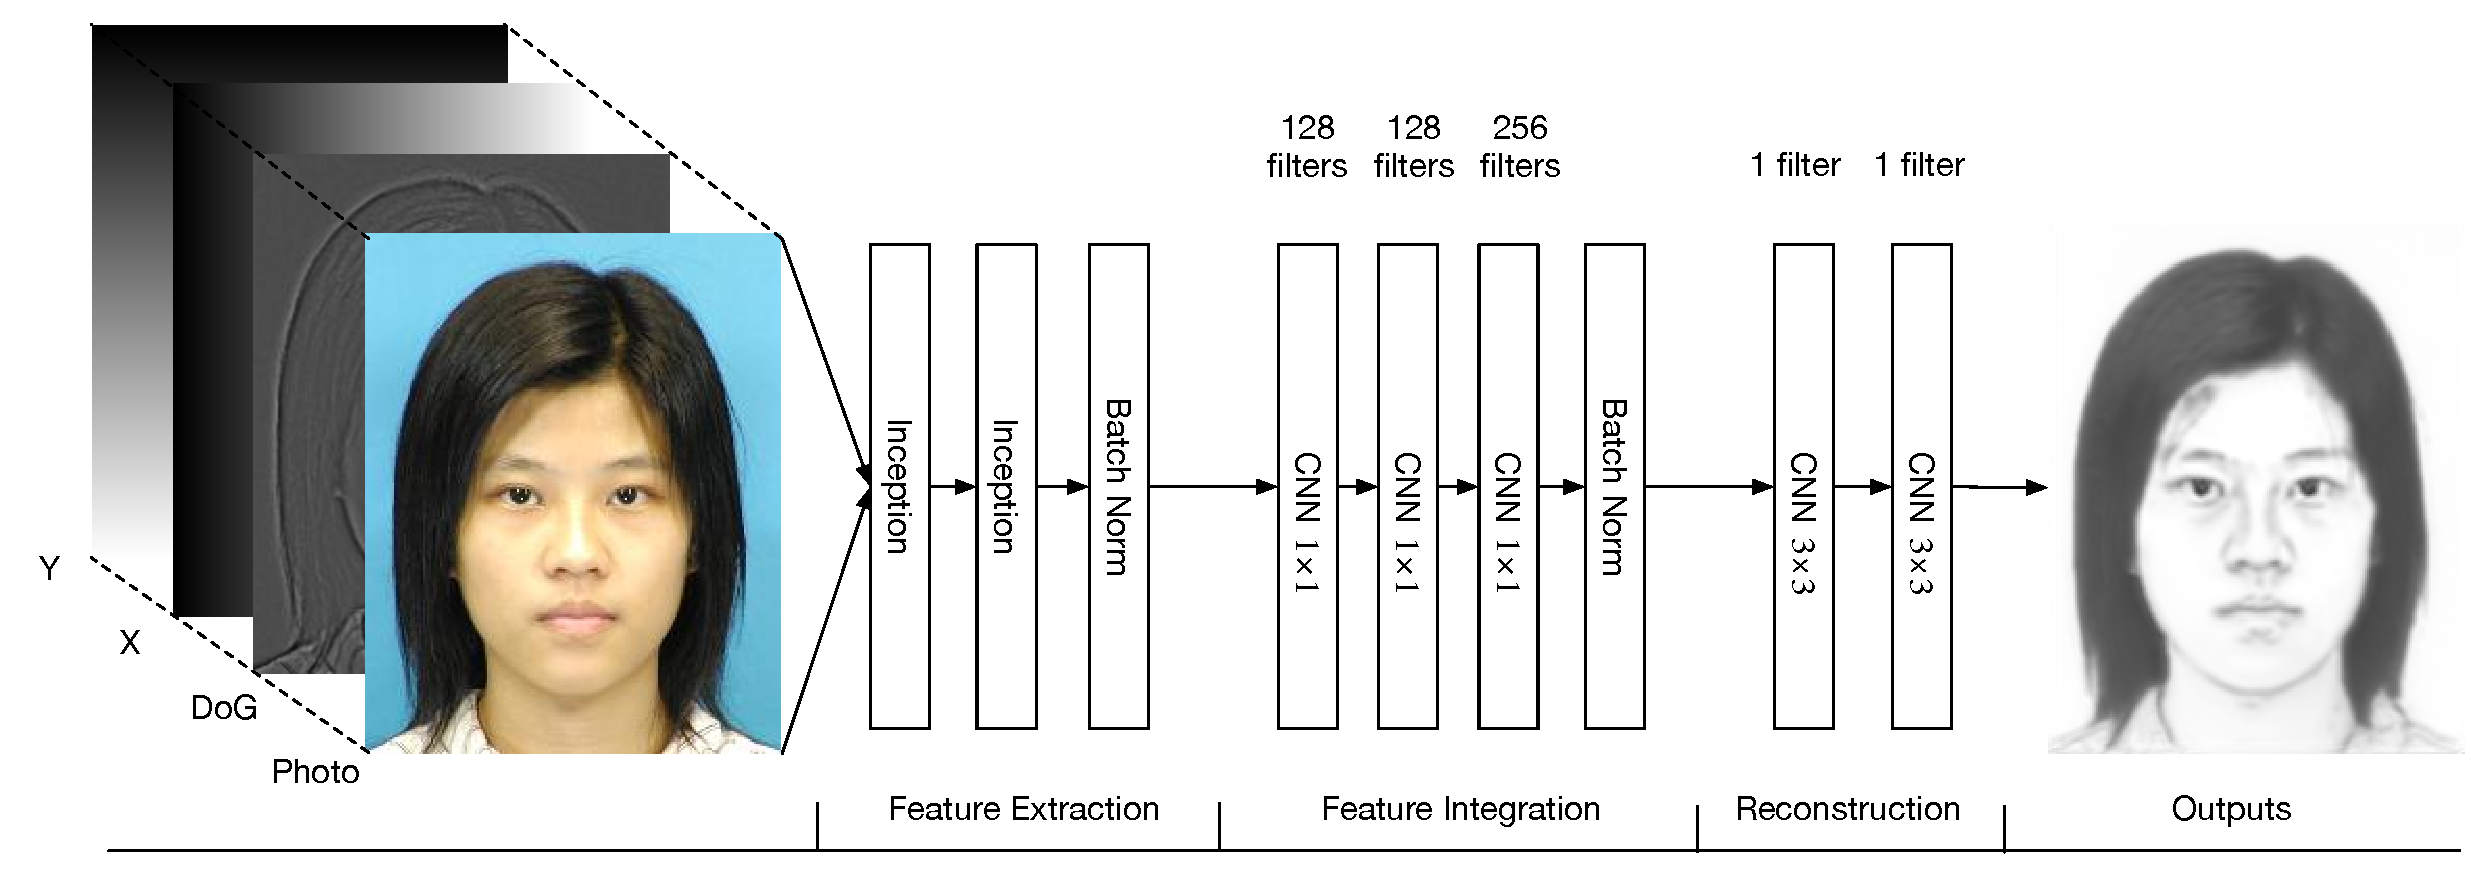
\includegraphics[width=0.65\linewidth]{content_net.pdf}
% }
% \subfigure[]{
% 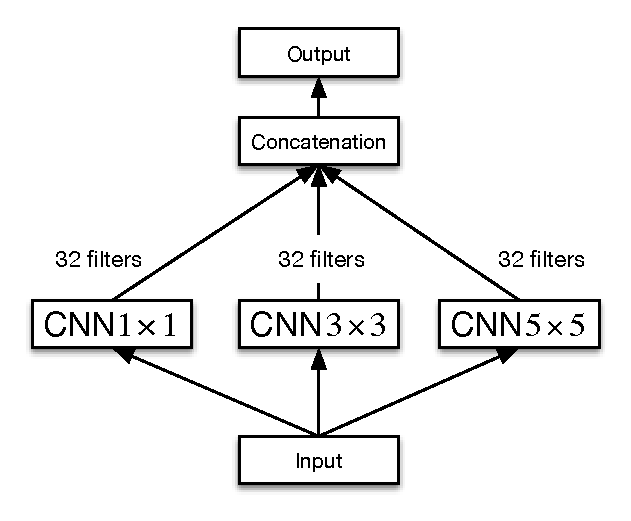
\includegraphics[width=0.25\linewidth]{inception.pdf}
% }
% \caption{Illustration of the content network for generating a content image. The numbers above the building block denote the number of CNN filters. (a) The architecture of content network. (b) The inception module in (a) contains three groups of filters with different sizes.}
% \label{fig:content_NN}
% \end{figure*}

{
\section{Sketch Style Generation}
}
{
\subsection{Style Representation}
}
The style features of sketches are extracted using the VGG-Network~\cite{simonyan2014very}, a CNN that was originally designed for visual object recognition tasks, and was later used for texture feature representation in~\cite{gatys2015texture}. Here we use the intermediate feature maps extracted by the convolutional layers and max-pooling layers in the VGG-19 network just before the fully connected layers. 

In the VGG-Network, convolutional layers extract features and max-pooling layers down-sample the features such that the following convolutional layers extract features in a lower resolution. We extract the outputs of the first convolutional layers at different resolutions for the computation of style. Following the terminology in~\cite{gatys2015texture}, these layers are referred to as ``conv1\_1'', ``conv2\_1'', ``conv3\_1'', ``conv4\_1'', and ``conv5\_1'', respectively, from the lowest level to the highest level. Define $L_s$ $=$ \{conv1\_1, conv2\_1, conv3\_1, conv4\_1, conv5\_1\}. Since the VGG-Network is originally designed for color images, while sketches are gray scale images, we modify the first layer of VGG-Network for gray scale images by setting the filter weights to
\begin{equation}
W^{k} = W^{k}_r+W^{k}_g+W^{k}_b
\label{eq:VGG_weights}
\end{equation}
where $W^{k}_r$, $W^{k}_g$, and $W^{k}_b$ are weights of the $k$th filter in the first convolutional layer for the R, G and B channels respectively, and $W^{k}$ is the weight of the $k$th filter in the first convolutional layer of our modified network. Note that we keep the bias in our modified network the same as that in the original VGG-Network. Denote the feature map of the final sketch $\mathcal{X}$ in the $l$th layer (in matrix form) by $F^{l}autoref(\mathcal{X})$, where the element at the $m$th row and the $n$th column is the activation of the $m$th filter at location $n$. We use the gram matrix as our style representation. A gram matrix is a summary statistics of feature maps discarding the spatial information, and  is originally designed for texture synthesis~\cite{gatys2015texture}. The gram matrix at layer $l$ is given by:
\begin{equation}
G^lautoref(\mathcal{X}) = {F^lautoref(\mathcal{X})} \cdot {autoref( {{F^lautoref(\mathcal{X})}} )^T}
\label{eq:Gram_element}
\end{equation}
where ${G^lautoref(\mathcal{X})} \in {\mathcal{R}^{{M_l} \times {M_l}}}$, and $M_l$ denotes the number of filters in layer $l$. A multi-resolution style representation is obtained by combining the gram matrices at different layers: $\mathcal{S}autoref(\mathcal{X})=$\{$G^l autoref(\mathcal{X})$\} where $l\in$\{conv1\_1, conv2\_1, conv3\_1, conv4\_1, conv5\_1\}. This style information is useful in guiding the sketch synthesis, especially in the texture region such as hair and shadings around the nose, eyes and mouth. 
{
\subsection{Target Style Generation via Multi-resolution Grouping}
}
% \begin{figure}[htbp]
% \centering
% 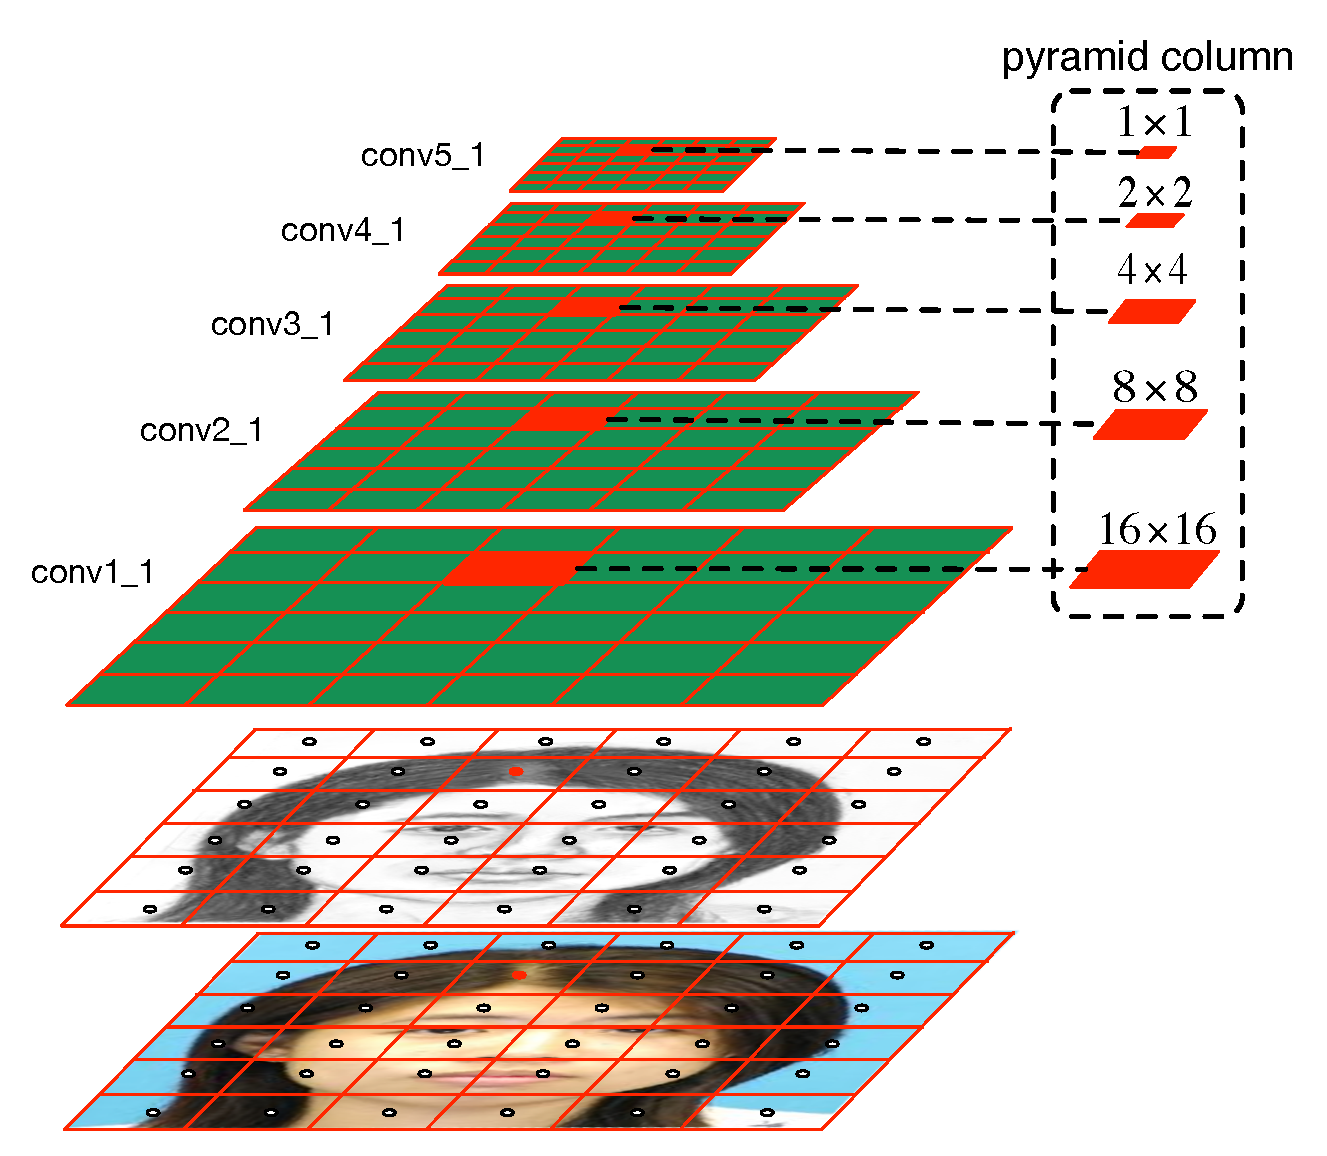
\includegraphics[width=0.85\linewidth]{pyramidcolumn.pdf}
% \caption{Illustration of pyramid column. Feature maps of the final sketch, $A^{l}$, are divided into patches according to the size of the smallest feature map. A pyramid column $U_{ij}$ consists of feature map patches at different layer having the same grid indices $i$ and $j$. The input photo and the final sketch are divided into patches where centers $C_{ij}$ are denoted as dots. $U_{12}$ and $C_{12}$ are colored in red as an example.}
% \label{fig:pyramidcolumn}
% \end{figure}
There usually does not exist a candidate image in the training set that perfectly matches a given test photo in style. We hence propose a patch based method to estimate the style of the final sketch. Denote the feature maps (of the $l$th layer) used to estimate the style of the final sketch by $A^{l}$. In our patch based method, we divide $A^{l}$ into a grid where each grid cell (feature map patch) at layer $conv5\_1$ contains only one pixel. Since the pooling size is $2\times2$, we choose the sizes of feature map patches at the next lower layer twice of that at the current layer. Thus, the sizes of the feature map patches at layer $conv1\_1$, $conv2\_1$, $conv3\_1$, $conv4\_1$ and $conv5\_1$ are $16\times16$, $8\times8$, $4\times4$, $2\times2$ and $1\times1$, respectively. We introduce a multi-resolution feature descriptor by grouping feature map patches having the same grid indices $i$, $j$ at different layer index $l$ together as a pyramid column, $U_{ij}$. The photos and sketches are resized so that both the number of rows and columns are dividable by $16$. $A^{l}$ can then be represented as a hyper-grid $U$ with the cells being $U_{ij}$. Similarly, we divide the test photo and the final sketch, respectively, into a grid with the same dimension as $U$. Denote the centers of these patches as $C_{ij}$. $U_{ij}$ is hence a multi-resolution feature descriptor for a sketch region centered at $C_{ij}$ (see Fig.~\ref{fig:pyramidcolumn}). 
To estimate $U_{ij}$, a sketch patch in the training set is fed to the VGG-Network and a pyramid column is composed from the resulting feature maps. This process consists of two steps: (1) find a matching sketch patch from the training set $S_{ij}$ for $U_{ij}$ and (2) feed $S_{ij}$ to VGG-Network and compose $U_{ij}$ from the resulting feature maps.\par
% \begin{figure*}[htbp]
% \centering
% \includegraphics[width=0.99\linewidth]{boarder_example.pdf}
% \caption{Find a matching patch for boarder cells. (a) The center $C_{ij}$ of a boarder cell is denoted as the red dot in the photo. (b) The region associated with $U_{ij}$ is the intersection of the blue square with the sketch. The distances between $C_{ij}$ to the intersection boarders are denoted by green lines. (c) $\tilde{C}_{ij}$ denoted as a yellow dot is located by examining photo similarity. (d) The distances of $\tilde{C}_{ij}$ to boarders of $S_{ij}$ equal to the distances of  $C_{ij}$ to boarders of intersection region in (b) such that the location of $\tilde{C}_{ij}$ in $S_{ij}$ is the same as the location of $C_{ij}$ in the region associated with $U_{ij}$.}
% \label{fig:boarder_example}
% \end{figure*}

{\noindent \bf Find Matching Sketch Patch}\\
Inspired by previous works~\cite{wang2009face,zhou2012markov}, we examine the similarity in appearance of photo patches to find a matching sketch $S_{ij}$ for $U_{ij}$. Denote a patch centered at $C_{ij}$ in the test photo as $\Psi_{ij}$. If a patch centered at $\tilde{C}_{ij}$ in the $k$th photo in the training set has the smallest Euclidean distance from $\Psi_{ij}$ in term of color channels, a sketch patch, $S_{ij}$, centered at $\tilde{C}_{ij}$ is extracted from the sketch paired with the $k$th photo in the training set. The size and position of $S_{ij}$ are determined by the region associated with $U_{ij}$ which is calculated according to the architecture of the VGG-Network and location of $C_{ij}$. For non-boarder cells, $S_{ij}$ is a sketch patch of size $144\times144$ centered at $\tilde{C}_{ij}$. For cells near boarders, the region associated with $U_{ij}$ is the intersection of a sketch patch of size $144\times144$ centered at $C_{ij}$ with the whole sketch. Therefore, $S_{ij}$ is a patch from the $k$th sketch containing $\tilde{C}_{ij}$ such that the location of $\tilde{C}_{ij}$ in $S_{ij}$ is the same as the location of $C_{ij}$ in the region associated with $U_{ij}$ (see Fig.~\ref{fig:boarder_example}).\\
{\bf Estimate Pyramid Column}\\
We compose an estimate for $U_{ij}$ from the resulting feature maps obtained by feeding $S_{ij}$ to the VGG-Network. Specifically, after feeding $S_{ij}$ to the VGG-Network, we form a hyper-grid $\tilde{U}$ on the resulting feature maps. The pyramid column corresponding to $\tilde{C}_{ij}$ is selected as an estimation to $U_{ij}$. This pyramid column is the cell that contains $\tilde{C}_{ij}$ when projecting $S_{ij}$ onto $\tilde{U}$.\par
After $A^{l}$ are estimated, we calculate the target gram matrices by: \{$G_{t}^l =A^{l} \cdot {autoref( {{A^{l}}} )^T}$\} where $l\in L_s$.

{
\section{Combine Style with Content}
}
To generate a sketch that combines the content image with the estimated style, we adopt the methodology described in~\cite{gatys2015texture}. Specifically, we minimize a loss function consisting of a style loss, a content loss and a component loss. The style loss is defined as the difference between the gram matrix of the final sketch and the target gram matrix i.e.,
\begin{equation}
\mathcal{L}_{s} autoref( \mathcal{X} ) = \sum\limits_{l \in {L_s}} {\frac{1}{{M_l^2N_l^2}}autoref\| {{G^l}autoref( \mathcal{X} ) - G_t^l} \|_2^2} 
\label{eq:Gram_loss}
\end{equation}
where $N_l$ denotes the number pixels in the feature map at layer $l$. The content loss is defined based on the difference between the feature map of the sketch and that of the content image at layer conv1\_1:
\begin{equation}
\mathcal{L}_{c}autoref( \mathcal{X} ) = autoref\| {{F^{\rm{conv1\_1}}}autoref( \mathcal{X} ) - {F^{\rm{conv1\_1}}}autoref( \mathcal{C} )} \|_2^2.
\label{eq:Style_loss}
\end{equation}
Human is able to distinguish different people from key components such as eyes, nose and mouth, which indicates that these features are the most discriminative parts of a face. Specific styles or textures are usually used to emphasize these components, for example, sharp edges with shadings at the two sides of the nose are used to convey 3D information. To better transfer styles of these components, we employ a component loss to encourage the key component style of the final sketch being the same as the target key component style. Since two eyes are placed at fixed positions, the key components lie roughly within a rectangular region taking the positions of two eyes as vertices. Key component style is given by gram matrices calculated within feature map regions $\mathcal R$ corresponding to the key components. These regions are specified by hyper-grid cells $U_{ij}$ whose $C_{ij}$ are inside the rectangular region. More specifically, a target style for the key component is calculated: \{${\hat G}_{t}^l ={A}_{c}^l \cdot {autoref( {{{A}_{c}^l}} )^T}$\} where ${A}_{c}^l$ is the composed feature map patch in $A^{l}$ corresponding to the key components, $l\in L_s$. The style of the key components in final sketch ${\hat G}^lautoref( \mathcal{X} ) $ is calculated in exactly the same manner. The component loss is hence defined as:
\begin{equation}
\mathcal{L}_{k} autoref( \mathcal{X} ) = \sum\limits_{l \in {L_s}} {\frac{1}{{M_l^2{\hat N}_l^2}}autoref\| {{{\hat G}^l}autoref( \mathcal{X} ) - {\hat G}_t^l} \|_2^2} 
\label{eq:component_loss}
\end{equation}
where ${\hat N}_l$ denotes the number of pixels in the feature map region $\mathcal R$ at layer $l$. The total loss we minimize is 
\begin{equation}
\mathcal{L}_{t}autoref( \mathcal{X} ) = \alpha \mathcal{L}_{c} + \beta_1 \mathcal{L}_{s} + \beta_2 \mathcal{L}_{k}
\label{eq:Total_loss}
\end{equation}
where $\alpha$, $\beta_1$ and $\beta_2$ are the weighting factors for content, style and component losses respectively. The minimization is carried out using L-BFGS. Instead of using random noises, we use the content image as a starting point, which will make the optimization process converge much faster. 
{
\section{Experiments}
}
% \begin{figure*}[htbp]
% \centering
% \begin{minipage}[t]{0.245\linewidth}
% \centering
% 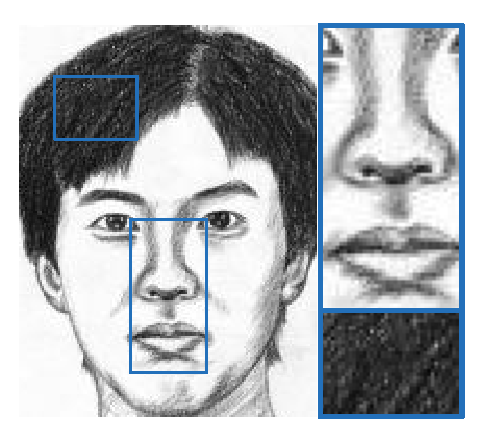
\includegraphics[width=0.99\linewidth]{example1_gro.pdf}
% 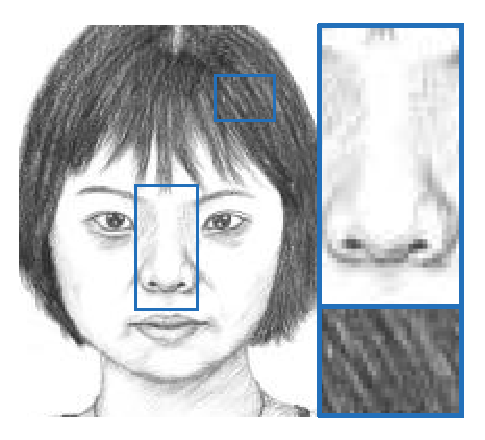
\includegraphics[width=0.99\linewidth]{example2_gro.pdf}
% (a) Sketches by artist
% \end{minipage}
% \begin{minipage}[t]{0.245\linewidth}
% \centering
% 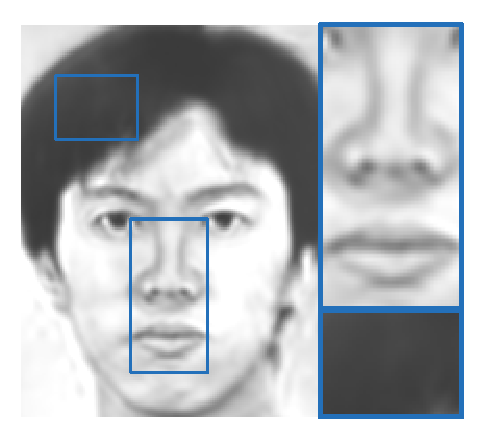
\includegraphics[width=0.99\linewidth]{example1_FCNN.pdf}
% 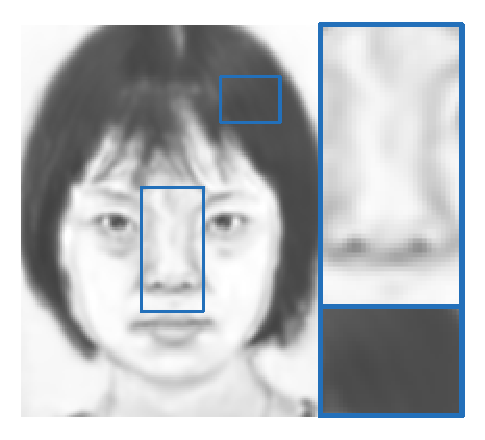
\includegraphics[width=0.99\linewidth]{example2_FCNN.pdf}
% (b) FCNN
% \end{minipage}
% \begin{minipage}[t]{0.245\linewidth}
% \centering
% 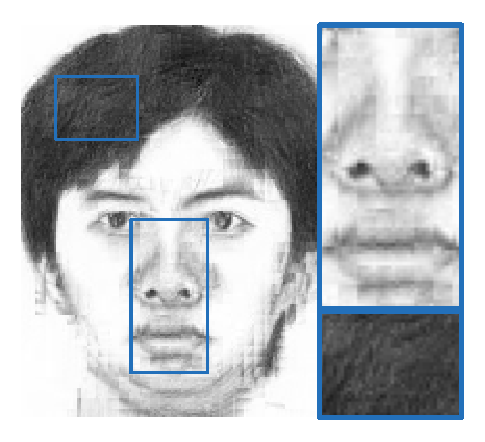
\includegraphics[width=0.99\linewidth]{example1_MRF.pdf}
% 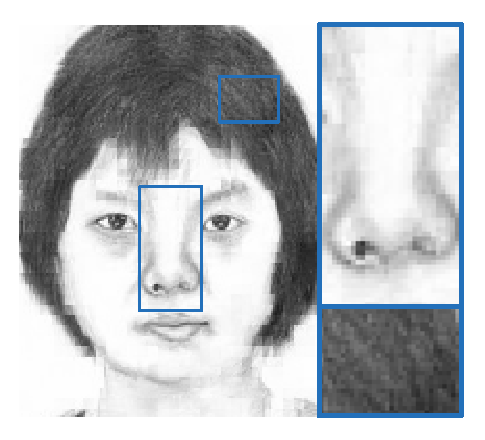
\includegraphics[width=0.99\linewidth]{example2_MRF.pdf}
% (c) MRF
% \end{minipage}
% \begin{minipage}[t]{0.245\linewidth}
% \centering
% 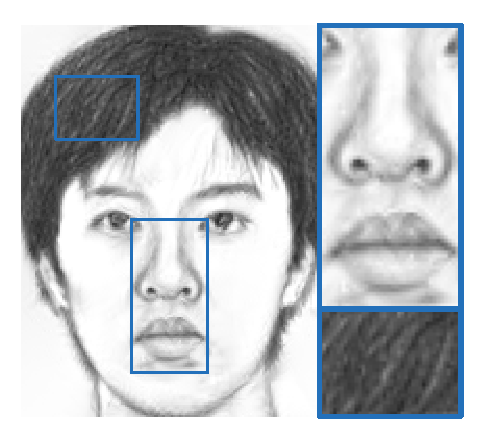
\includegraphics[width=0.99\linewidth]{example1_ours.pdf}
% 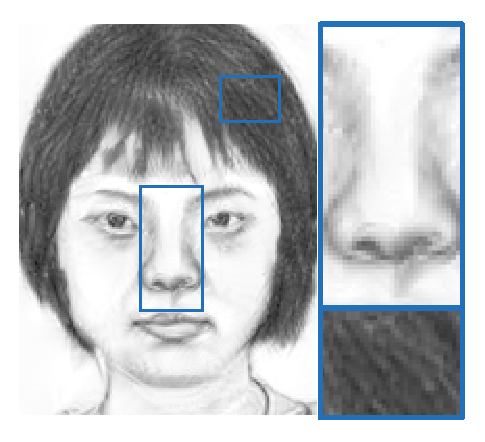
\includegraphics[width=0.99\linewidth]{example2_ours.pdf}
% (d) Ours
% \end{minipage}
% \caption{Examples of qualitative evaluation on CUHK benchmark datasets. (a) The sketches drawn by artists. (b) Results from feed-forward CNN based method~\cite{zhang2015end}. (c) Results from MRF based method~\cite{wang2009face}. (d) Our results.}
% \label{fig:q_eval_1}
% \end{figure*}
% \begin{figure*}[htbp]
% \centering
% \begin{minipage}[t]{0.245\linewidth}
% \centering
% 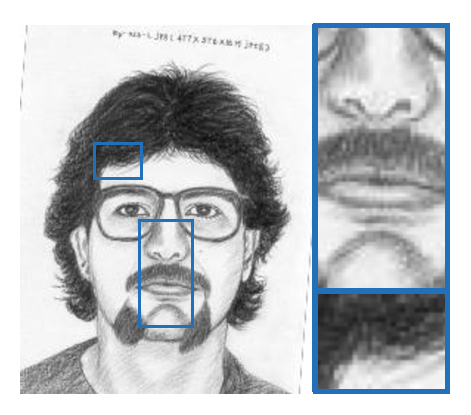
\includegraphics[width=0.99\linewidth]{example3_gro.pdf}
% 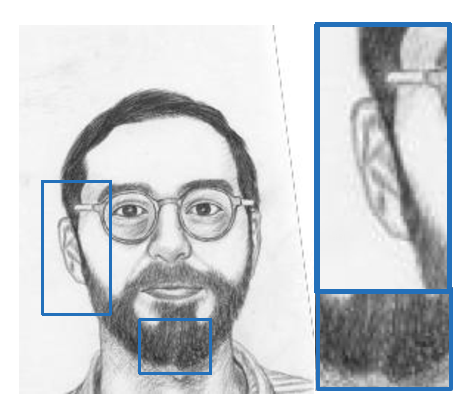
\includegraphics[width=0.99\linewidth]{example4_gro.pdf}
% (a) Sketches by artist
% \end{minipage}
% \begin{minipage}[t]{0.245\linewidth}
% \centering
% 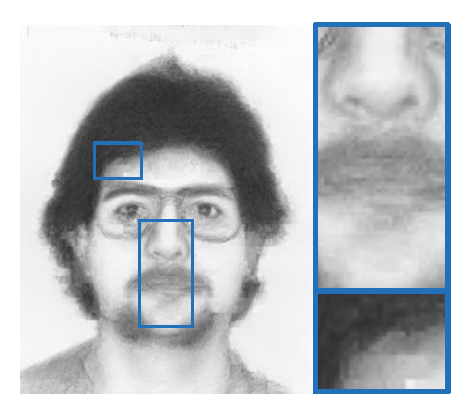
\includegraphics[width=0.99\linewidth]{example3_WMRF.pdf}
% 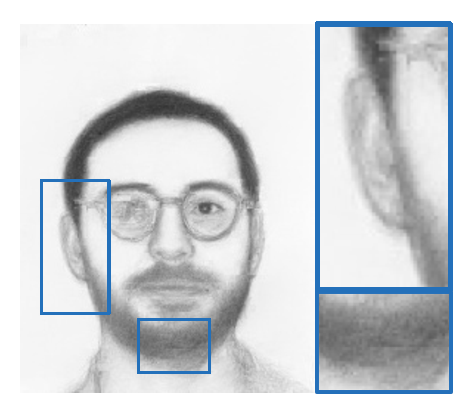
\includegraphics[width=0.99\linewidth]{example4_WMRF.pdf}
% (b) WMRF
% \end{minipage}
% \begin{minipage}[t]{0.245\linewidth}
% \centering
% 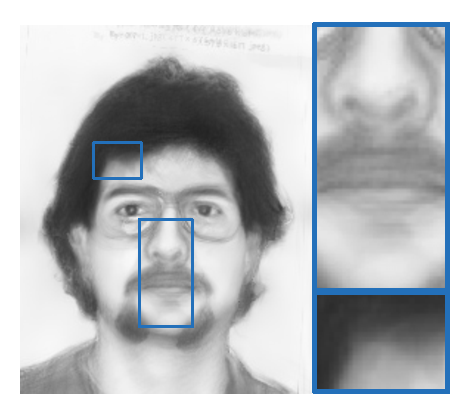
\includegraphics[width=0.99\linewidth]{example3_Filter.pdf}
% 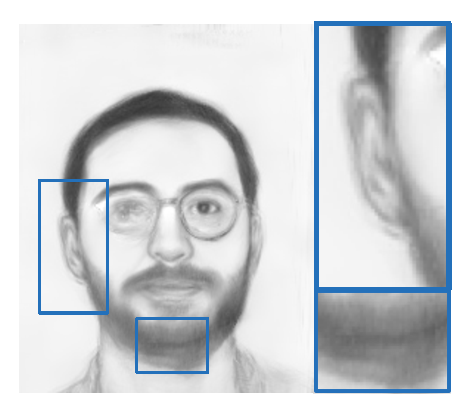
\includegraphics[width=0.99\linewidth]{example4_Filter.pdf}
% (c) SSD
% \end{minipage}
% \begin{minipage}[t]{0.245\linewidth}
% \centering
% 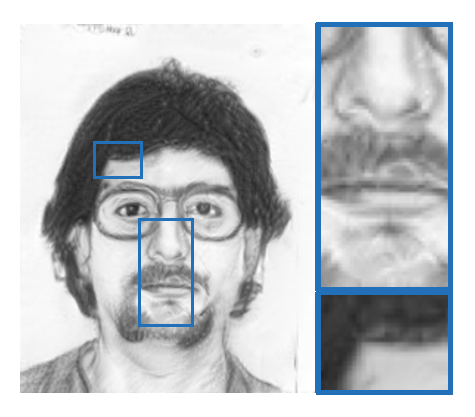
\includegraphics[width=0.99\linewidth]{example3_ours.pdf}
% 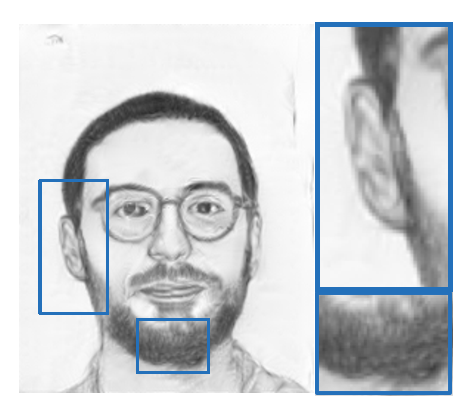
\includegraphics[width=0.99\linewidth]{example4_ours.pdf}
% (d) Ours
% \end{minipage}
% \caption{Examples of qualitative evaluation on AR benchmark datasets. (a) The sketches drawn by artists. (b) Results from the WMRF method~\cite{zhou2012markov}. (c) Results from the SSD method~\cite{song2014real}. (d) Our results.}
% \label{fig:q_eval_2}
% \end{figure*}
In all experiments, we resize test photos and photo-sketch pairs in the training set to a fixed size of $288\times288$. The final sketch is obtained by resizing the resulting sketch back to the original size. The size of $\Psi$ is $48\times48$, $\alpha=0.004$, $\beta_1=1$ and $\beta_2=0.1$. Since generating the final sketch involves an iterative optimization process, the gradient of the final sketch with respect to the content image is not easy to calculate, which prohibits training the content network in an end-to-end manner.  The training is therefore carried out by minimizing the squared loss between generated content images and sketches drawn by artists. We evaluate the performance of the proposed method against other state-of-the-art methods on the CUHK student dataset~\cite{wang2009face} and the AR dataset~\cite{martinez1998r}. For AR dataset, we use the leave-one-out strategy as conducted in previous studies~\cite{song2014real,wang2009face}. We compare the results of our method against those of the MRF method~\cite{wang2009face}, weighted MRF (WMRF) method~\cite{zhou2012markov}, feed-forward CNN (FCNN) method~\cite{zhang2015end} and Filtering based method (SSD)~\cite{song2014real}.
{
\subsection{Sketch Recognition}
}
Sketch synthesis methods are usually evaluated quantitatively  via the face sketch recognition task~\cite{song2014real,wang2009face,zhang2015end,zhou2012markov}. If an algorithm achieves higher sketch recognition rates, it suggests that this method is more effective in synthesizing sketches. We adopt the widely used PCA based recognition method with ``rank-1 (R1)'', ``rank-5 (R5)'' and ``rank-10 (R10)'' criteria ~\cite{wang2009face} where ``rank $n$'' measures the rate of the correct answer in the top $n$ best matches. The results of different methods are shown in Table~\ref{tab:reg_percentage}. Our method achieves the best performance against all other methods in the ``R1'' and ``R5'' tests. There may be two reasons behind this. First, since the test photos are different from those in the training set, we do not expect to find suitable patches from the training set for the target patches. The remedy of linearly combining the patches as in~\cite{zhou2012markov} will introduce over smoothing and blurring artifacts, which are also observed in the filtering like approach~\cite{song2014real}. Being a generative model, the content network learns the modality transformation locally between photos and sketches, such as transferring edges in photos to strokes in sketches. This helps generating sketches for structures not existing in the training set. Second, our model explicitly minimizes the difference by the style between the synthesized sketches and sketches drawn by artists, while this difference is ignored by all other methods. The performance of all methods in the ``R10'' test are fairly the same. 
\begin{table}
\small
\begin{tabular}{C{0.2cm}C{0.2cm}C{0.35cm}C{0.1cm}C{0.35cm}C{0.1cm}C{0.35cm}C{0.1cm}C{0.35cm}C{0.1cm}C{0.35cm}C{0.1cm}C{0.35cm}}
\hline
\multicolumn{2}{c|}{\multirow {2}{*}{Methods}} & \multicolumn{5}{c}{AR} & & \multicolumn{5}{c}{CUHK} \\
\cline{3-7} \cline{9-13} \multicolumn{2}{c|}{} & R1 & & R5 & & R10 & & R1 & & R5 & & R10   \\
\hline
\multicolumn{2}{c|}{FCNN} & - & & - & & - & & 81\% & & 96\% & & 97\%   \\
\multicolumn{2}{c|}{MRF}  & 97.5\% & & 97.5\% & & \textcolor{red}{100\%} & & 83\% & & 96\% & & 96\% \\
\multicolumn{2}{c|}{WMRF} & 97.5\% & & 97.5\% & & \textcolor{red}{100\%} & & 83\% & & 97\% & & 98\%  \\
\multicolumn{2}{c|}{SSD}  & 96.7\% & & 97.5\% & & \textcolor{red}{100\%} & & \textcolor{red}{87\%} & & 97\% & & 98\%   \\
\multicolumn{2}{c|}{Ours} & \textcolor{red} {98.4\%} & & \textcolor{red} {98.4\%} & & \textcolor{red} {100\%} & & \textcolor{red} {87\%} & & \textcolor{red} {98\%} & & \textcolor{red} {99\%}   \\
\hline
\end{tabular}
\caption{Recognition rate on benchmark datasets. The best performance is colored in red.}
\label{tab:reg_percentage}
\end{table}

\begin{table*}[htbp]
\begin{center}
{\small
\begin{tabular}{ccccccccccccc}
\hline
\multicolumn{2}{c|}{\multirow {2}{*}{Methods}} &\multicolumn{5}{c}{AR} & & \multicolumn{5}{c}{CUHK} \\
\cline{3-7} \cline{9-13} \multicolumn{2}{c|}{} & conv1\_1 & conv2\_1 & conv3\_1 & conv4\_1 & conv5\_1 & &
 conv1\_1 & conv2\_1 & conv3\_1 & conv4\_1 & conv5\_1  \\
\hline
\multicolumn{2}{c|}{FCNN} & - & - & - & - & - & & { $0.009$} &{ $0.110$} & {$0.080$} & {$9.43$} & {$1.49$}  \\
\multicolumn{2}{c|}{MRF} & 0.0043 & 0.009 & {$0.033$}  & {$0.12$} & 0.28 & & { $0.010$} &{ $0.014$} & {$0.047$} & $0.13$ & $0.18$  \\
\multicolumn{2}{c|}{WMRF} & 0.0053 & 0.027 & {$0.085$}  & {$0.19$} & 0.29 & & { $0.010$} &{ $0.052$} & {$0.052$} & {$0.27$} & {$0.19$}  \\
\multicolumn{2}{c|}{SSD} & 0.0056 & 0.036 & {$0.110$} & {$1.90$} & 0.28 & & { $0.009$} &{ $0.102$} & {$0.070$} & {$3.32$} & {$0.24$}  \\
\multicolumn{2}{c|}{Ours} & {\color{red} 0.0035} & {\color{red} 0.008} & {\color{red} $0.029$} & {\color{red} $0.08$} & {\color{red} $0.17$} & & {\color{red}$0.007$} &{\color{red} $0.012$} & {\color{red} $0.033$} & {\color{red} $0.07$} & {\color{red} $0.12$}  \\
\hline
\end{tabular}
}
\end{center}
\caption{Averaged NGMD value of different methods at different level on AR and CUHK datasets.}
\label{tab:NGMD}
\end{table*}
{
\subsection{Style Transfer}
}
% \begin{figure}[htbp]
% \centering
% \begin{minipage}[t]{0.49\linewidth}
% \centering
% 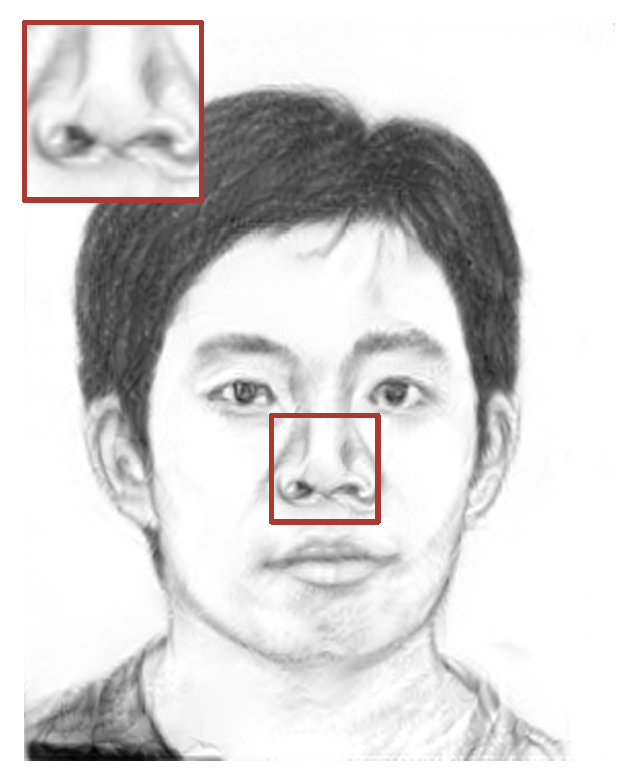
\includegraphics[width=0.99\linewidth]{wo_region.pdf}
% (a) $\beta_2=0$
% \end{minipage}
% \begin{minipage}[t]{0.49\linewidth}
% 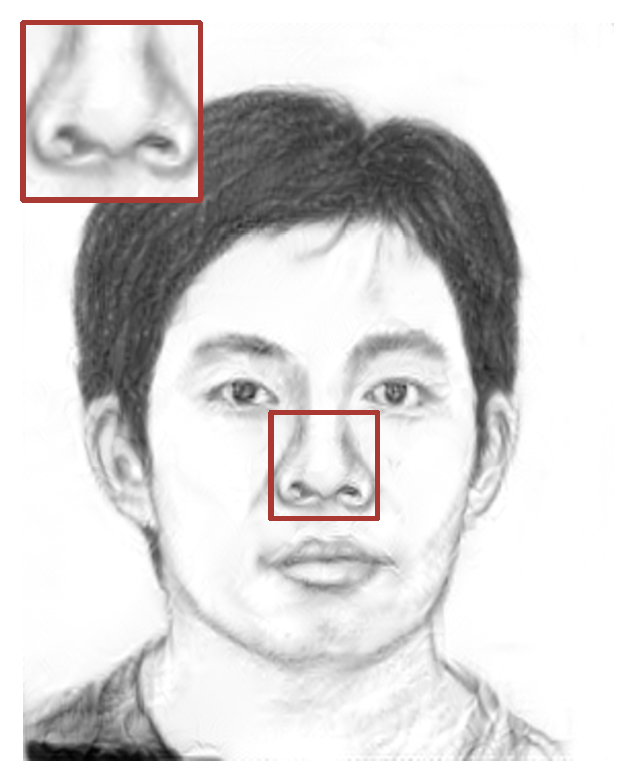
\includegraphics[width=0.99\linewidth]{w_region.pdf}
% \centering
% (b) $\beta_2=0.1$
% \end{minipage}
% \caption{Comparison between results with and without the $\mathcal{L}_{k} $ regulation. (a) When turning off the component loss, the nose suffers from the distortion. (b) Thanks to the component loss, a more favorable result is obtained.}
% \label{fig:region_effect}
% \end{figure}

% \begin{figure*}[htbp]
% \centering
% \begin{minipage}[t]{0.16\linewidth}
% \centering
% 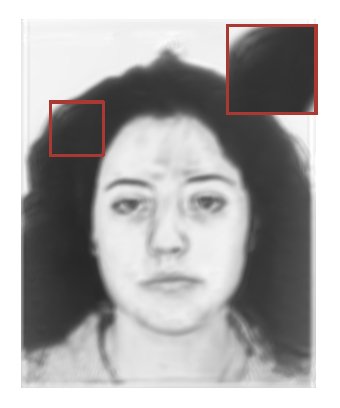
\includegraphics[width=0.99\linewidth]{inf_alpha.pdf}
% $\beta_1  = 0 $\\
% $\beta_2  = 0 $
% \end{minipage}
% \begin{minipage}[t]{0.16\linewidth}
% \centering
% 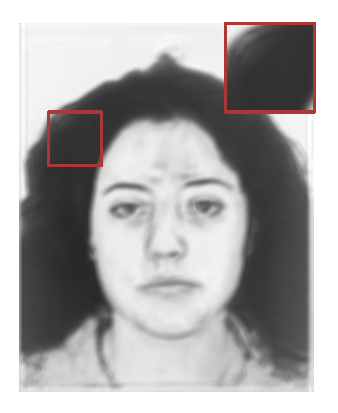
\includegraphics[width=0.99\linewidth]{4_alpha.pdf}
% $\beta_1  = 10^{-3} $\\
% $\beta_2  = 10^{-4} $
% \end{minipage}
% \begin{minipage}[t]{0.16\linewidth}
% \centering
% 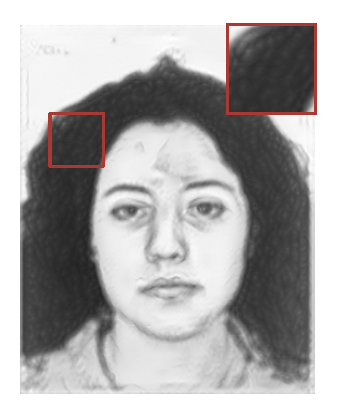
\includegraphics[width=0.99\linewidth]{3_alpha.pdf}
% $\beta_1  = 10^{-2} $\\
% $\beta_2  = 10^{-3} $
% \end{minipage}
% \begin{minipage}[t]{0.16\linewidth}
% \centering
% 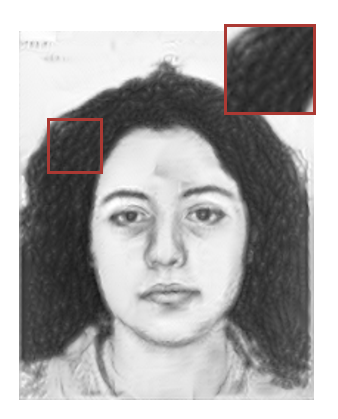
\includegraphics[width=0.99\linewidth]{2_alpha.pdf}
% $\beta_1  = 0.1 $\\
% $\beta_2  = 0.01 $
% \end{minipage}
% \begin{minipage}[t]{0.16\linewidth}
% \centering
% 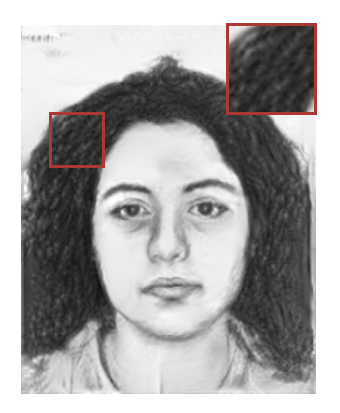
\includegraphics[width=0.99\linewidth]{1_alpha.pdf}
% $\beta_1  = 1 $\\
% $\beta_2  = 0.1 $
% \end{minipage}
% \begin{minipage}[t]{0.16\linewidth}
% \centering
% 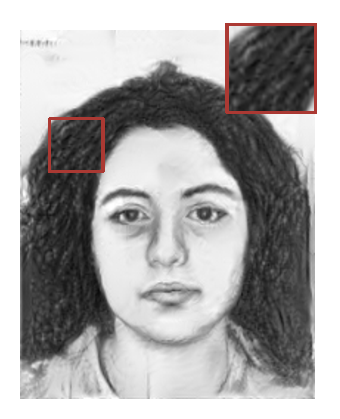
\includegraphics[width=0.99\linewidth]{0_alpha.pdf}
% $\beta_1  = 10^{3} $\\
% $\beta_2  = 10^{2} $
% \end{minipage}
% \caption{Final results for sketch synthesis with fixed $\alpha=0.004$ and different $\beta_1$, $\beta_2$ values.}
% \label{fig:alphg_effect}
% \end{figure*}
Human can often be able to tell whether a sketch is generated by algorithms or drawn by artists just from a quick glance without examining details. This indicates that there exists a big gap between the style of algorithm-generated sketches and that of those drawn by artists. To quantitatively evaluate the style similarity between a generated sketch and the sketch drawn by a real artist, we employ the normalized gram matrix difference (NGMD) between the generated sketch $\mathcal{X}$ and the drawn sketch ${\tilde {\mathcal{X}}}$:
\begin{equation}
{D^l_s}autoref( {\mathcal{X},\tilde {\mathcal{X}}} ) = \frac{{autoref\| {{G^l}autoref( \mathcal{X} ) - {G^l}autoref( {\tilde {\mathcal{X}}} )} \|_2^2}}{{autoref\| {{G^l}autoref( {\tilde {\mathcal{X}}} )} \|_2^2}}
\label{eq:style_exp}
\end{equation}
where $l\in L_s$. The smaller the NGMD value is, the more similar $\mathcal{X}$ and ${\tilde {\mathcal{X}}}$ are. Thanks to our style transfer, our results have the smallest NGMD value among all methods under test (see Table 2). It is therefore obvious that our results are the closest to the sketches drawn by artists. 
Qualitative evaluation results are shown in Fig.~\ref{fig:q_eval_1} and Fig.~\ref{fig:q_eval_2}, where we find that our method provides much clear boundaries and better texture in regions containing hairs and shadings. The results of~\cite{zhang2015end} can roughly outline the sketches, but they do not look like sketches in style. This is also indicated by a high NGMD in Table~\ref{tab:NGMD}. The results of MRF~\cite{wang2009face} and WMRF~\cite{zhou2012markov} are more similar to hand drawn sketches in style since these exemplar based approaches use patches of hand drawn sketches to make up the target sketch. That is why they have a smaller NGMD value. Inheriting the ability of denoising, the filtering based approach~\cite{song2014real} is good at suppressing noises in the results. However, it is also likely for this method to over-smooth the results, which will deteriorate the texture and even introduce blurring artifacts. 
{
\subsection{Effectiveness of the model}
}
The loss function we minimize during the generation of sketches contains three terms for content, style and key components respectively. The term $\mathcal{L}_{k} $ regularizes the results by encouraging the style extracted from the key component regions in the training set to be placed into the key components region of the results, which helps generate better results around these components (see Fig.~\ref{fig:region_effect}). To better understand how style influences the final sketch, we smoothly change the emphasis on style by adjusting $\beta_1$ and $\beta_2$ while keeping $\alpha$  fixed. Fig.~\ref{fig:alphg_effect} indicates that the sketch with style transfered contains more texture and is more like a drawn sketch. The Theano implementation of the proposed method takes approximately $100$ seconds to generate a sketch on a GeForce GTX TITAN X platform. The bottle neck lies in the style transfer which requires feeding $\mathcal{X}$ to the VGG-Network to estimate targeting feature maps and to calculate the gradient of Eq.~(\ref{eq:Total_loss}), which is computationally intensive. 
{
\section{Conclusion and Future Work}
}
This paper proposed a novel face sketch synthesis method inspired by the procedure of artists drawing sketches. In our method, the outline of the face is delineated by a content network and the style extracted from sketches drawn by artists are transferred to generate a final sketch. Quantitative evaluations on face sketch recognition and style similarity measure demonstrate the effectiveness of the proposed algorithm for face sketch synthesis and style transferring. Our future work will investigate accelerating technique to reduce the running time and achieve real time face sketch synthesis with style transfer.


{\small
\bibliographystyle{ieee}
\bibliography{egbib}
}

\end{document}